%!TEX root = ../thesis.tex

\begin{savequote}[70mm]
	It is one thing to mortify curiosity,\\another to conquer it.
	\qauthor{Robert Louis Stevenson, Dr. Jekyll and Mr. Hyde }
\end{savequote}

\chapter{Background}\label{chapter:background}

	This chapter introduces the background concepts necessary to understand the project presented in this thesis and why it has been developed.
	
	It first explains the definition of IoT, afterwards, it describes the air pollution problem, to conclude with an overview on the background work and state or art of two devices capable of detecting pollutants in the air.

	Mesh networks are better described in Chapter \ref{chapter:related_work}, where also previously made projects which use a similar architecture are described.

	\section{Internet of Things}
	
		%https//www.smithsonianmag.com/innovation/kevin-ashton-describes-the-internet-of-things-180953749/
		%http://www.itrco.jp/libraries/RFIDjournal-That%20Internet%20of%20Things%20Thing.pdf
		%https://www.rfidjournal.com/that-internet-of-things-thing
		
		Internet of Things, also abbreviated with IoT, has a longer history than many people think about: its name, now know all around the globe, has been attributed to Kevin Ashton, who used it in a presentation about Radio Frequency Identification (RFID) technology, at \textit{Protector \& Gamble}, in 1999 \cite{iot_definition} to describe the network connecting objects in the physical world to the Internet.
		
		This constantly expanding branch of Computer Science aims to turn physical objects, as small as they may be, into nodes of an interconnected system which opens the door to new interfaces between humans and machines and how these see the physical world.
		IoT's importance heavily relies on data gathered from these devices, since, in combination with other computer science paradigms such as Machine Learning and Artificial Intelligence, raw data can be transformed into valuable information.
	
		The creation of models from all these inputs has given a more efficient workflow in companies and has improved certain aspects of everyday life, from wearable technologies to Inter-Vehicular Communication (IVC).
		As explained in \cite{BUJARI2020101204}, the latter is a ``\textit{key technology in order to increase driving efficiency and safety, as well as	support autonomous driving and provide many other connectivity-based services}''.
		The biggest challenges though are \textit{heterogeneity} of devices and \textit{dynamicity} in vehicular scenarios.
		
		Another important application scenario of IoT is emergency situations, where it supports first responders with adequate means to perform their operations in a safe  and effective way.
		In this case, from a networking point of view, ``\textit{one of the main challenges is that of providing first responders with multimedia information about the emergency as soon as possible, even from a remote location}'' \cite{4197976}.
		Projects designed to provide connectivity off-grid not only to civilians, but firefighters, military operations, local law enforcement, search and rescue, are described in Section \ref{sec:chap4_projects}.

		But first, below are two important key projects in the story of IoT the UPC, or Universal Product Code, and the Carnegie Mellon University (CMU) coke machine.
		
		\subsection{Universal Product Code and Barcode}
	
			% https://www.thoughtco.com/bar-codes-history-1991329
			One of the first technologies that can be considered part of the IoT family, is the ``\textit{Universal Product Code}'', or \textit{UPC}.
			Its first iteration is detailed in the patent issued to inventors Joseph Woodland and Bernard Silver on October 7, 1952, and can be described as a ``\textit{bull's eye}'' symbol, made up of a series of concentric circles \cite{upc_patent}, as can be seen in Figure~\ref{img:upc_patent}.
			
			\begin{figure}[h]
				\centering
				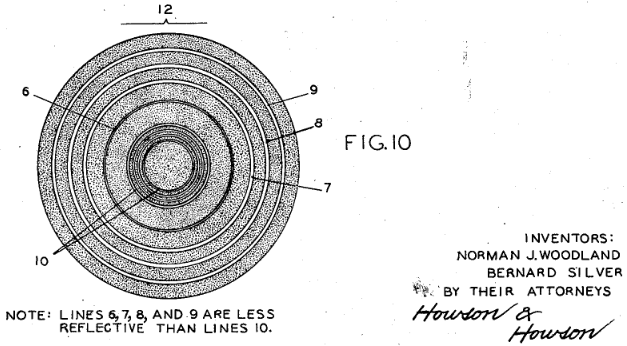
\includegraphics[width=\textwidth-4cm]{resources/img/chap2/upc_1}
				\caption[Diagrammatic view of the Universal Product Code]{Diagrammatic view of the Universal Product Code \cite{upc_patent}}
				\label{img:upc_patent}
			\end{figure}
			
			Authors of the patent, state  that ``\textit{one application of the invention is in the so called 'super-market' field}'', indicating they already successfully identified a need to speed up and automatizing the process of paying at super-markets.
			
			Due to the large size and low reliability of the equipment necessary to read the figure, this concept has not been immediately released for everyday use.
			Commercial adoption relied on the emergence of laser optics, which started to offer a more compact reading technology.
			
			Although, printers were vulnerable to smudge the design coped with errors as ink bleeding would result in taller bars.
			Thus, the ameliorated UPC print was vertical and came in the form of a barcode printed with strict rules in order to avoid errors in scanning due to smear or marks on the label.
			This version, developed in 1971 by George Laurer at IBM \cite{upc_ibm}, became the first wide appearance of the upc.
			
			A centralizes super-system that provided the code translations was used in order to standardize codes among different super markets and shopping places.
			Such system has been the first way to track products and address them at large scale, thus rendering a ``\textit{thing}'' at the super market capable of providing information to a larger scale, although not directly connected.
			
		\subsection{CMU's coke machine and modern vending machines}
	
			%https://www.engineersrule.com/how-a-coke-machine-and-the-industrial-internet-of-things-can-give-birth-to-a-planetary-computer/
			%https://www.ibm.com/blogs/industries/little-known-story-first-iot-device/
			%https://www.cs.cmu.edu/~coke/history_long.txt
		
			It may come as a surprise, but connecting everyday ``\textit{things}'' for direct interaction, contrary to the previous example, started around the 1980s.
			
			\noindent
			\begin{minipage}{0.5\textwidth}% adapt widths of minipages to your needs
				\centering
				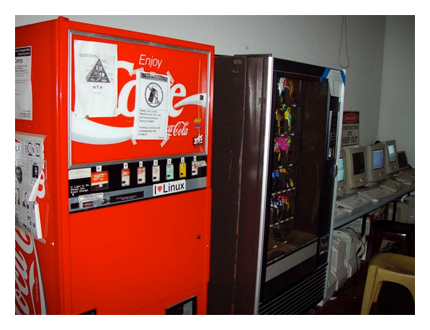
\includegraphics[width=\textwidth]{resources/img/chap2/coke}
				\captionof{figure}{CMU's ``\textit{coke machine}''}
			\end{minipage}%
			\hfill%
			\begin{minipage}{0.5\textwidth}\raggedright
				One of the most famous and most quoted as the first IoT device, is the Carnegie Mellon University (CMU) coke machine at the Computer Science Department.
				Communication from and to the machine, which allowed remote access, took place via Arpanet at CMU as the system predated the Internet.
				Various sensors were used to detect whether shelves were empty and to track status of coke bottles (warm, cold, empty).
			\end{minipage}
			\newline
			
			As explained in the official website\footnote{ \url{www.cs.cmu.edu/~coke/history_long.txt}} dedicated to this device by the University, there are ``\textit{micro-switches in the Coke machine to sense how many bottles were present in each of its six columns of bottles}''.
		
			Modern day vending machines usually require continuous connectivity to the manufacturer's systems.
			This is not always achievable via a Wi-Fi connection where machines are placed, so other solutions, such as cellular connectivity, are used.
			Connection reliability in vending machines and other kiosks is important since these provide goods that can be payed by credit card, which need to establish a secure connection.
			
			They contain multiple small, but complex, systems that interact with each other, thus it is implied that this kind of machines must have installed a secure software and that they need to be as hard as possible to be tampered with, either by brute force or by software bugs.
				
			Otherwise it is not only possible that someone steals a snack, but some remote script may turn these machines into a botnet capable of bringing down the connectivity of an entire campus.
			Such attack has been described in Verizon's ``\textit{Data Breach Digest}'' risk report from 2017, where the author states that ``\textit{the firewall analysis identified over 5,000 discrete systems making hundreds of DNS lookups every 15 minutes}'' \cite{DataBreachDigest}.
			
			While credit card skimmers and chip card cloners remain viable risks to the end consumer, security measures to the environment where machines are placed must not remain an afterthought, especially when these are placed alongside other connected devices and not in their own separated network.
			Such kind of smart vending machines have helped bring a step closer old ``\textit{un-connected}'' cities to become ``\textit{smart cities}'', where these machines can be used as a mean to place devices such as routers or public Wi-Fi access points.
	
		\subsection{Trends, forecasts and research directions}\label{sec:trends}
	
			IoT and related technologies have grown exponentially since the times of CMU's coke machine.
			According to data from Microsoft Academic\footnote{ \url{www.academic.microsoft.com/topic/81860439}}, publications about ``\textit{Internet of Things}'' have grown exponentially: from the 26 in the year 2000, to 534 in 2010, 4959 in 2015, to 22454 papers published in 2020.
			This shows how much interest IoT has gathered among the scientific community.
			Nonetheless, some IoT systems can still be considered not ready for mass deployment and many technical difficulties and problems need to be solved.
	
			Research directions in this new area are vast, since every physical device now represents a possible ``\textit{thing}'' connected in the network and that can be interacted with and provide data.
			Authors of \cite{9319033} have highlighted ten particular topic areas that span across three layers of IoT architecture: Application, Data and Physical, as represented in Figure~\ref{iot_research_areas}.
		
			\begin{figure}[h]
				\centering
				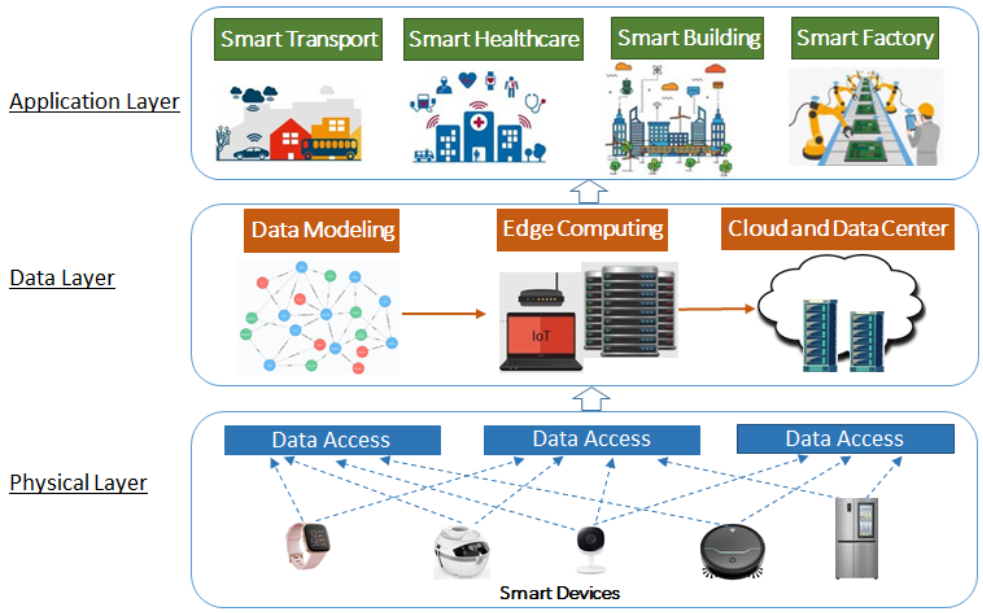
\includegraphics[width=0.9\textwidth]{resources/img/chap2/iot_research_areas}
				\caption[Most researched areas in IoT]{Most researched areas in IoT \cite{9319033}}
				\label{iot_research_areas}
			\end{figure}
		
			These topics include ``\textit{Data-driven IoT}'', ``\textit{Security, Privacy, and Trust in IoT}'', ``\textit{Social IoT}'', and ``\textit{Edge Computing and IoT}'', which have brought the need for new paradigms of computation.
			
			Data can be created and collected at a very high speed when considering the number of devices connected.
			This has been stimulating the creation of faster and more reliable database management systems (DBMSs) and brokers that allow higher processing speeds and querying frequencies.
			Specialized versions of these are emerging, each fitted for different scenarios, that may range from a fully online (or as a service with products such as AWS IoT Core\footnote{ \url{www.aws.amazon.com/iot-core/features}}) infrastructure to fully on premise one.
			
			Another important aspect is the network's architecture, which needs to take in consideration aspects such as heterogeneity of connected devices, velocity of data that flows across and scalability.
			Thus, paradigms like Cloud Computing, Fog Computing and Edge Computing\footnote{ ``\textit{Edge Computing does not mean computers at the edge of a table.}'' -cit. Alessandro Canesso} have emerged.
			
			% https://objectbox.io/what-is-edge-computing/
			% With Edge Computing, data stays where it is produced, used and where it belongs – without traversing the network unnecessarily.
			In Edge Computing, data points are used where they are produced, without traversing the network unnecessarily.
			This way, cloud infrastructure requirements are drastically reduced in three ways: firstly, less network traffic, secondly, less central storage and thirdly less computational power.
			Rather, Edge Computing makes use of all the capable hardware already deployed, e.g., in a smart home where all the data could stay within the house and be used on site.
			
			\begin{figure}[h]
				\centering
				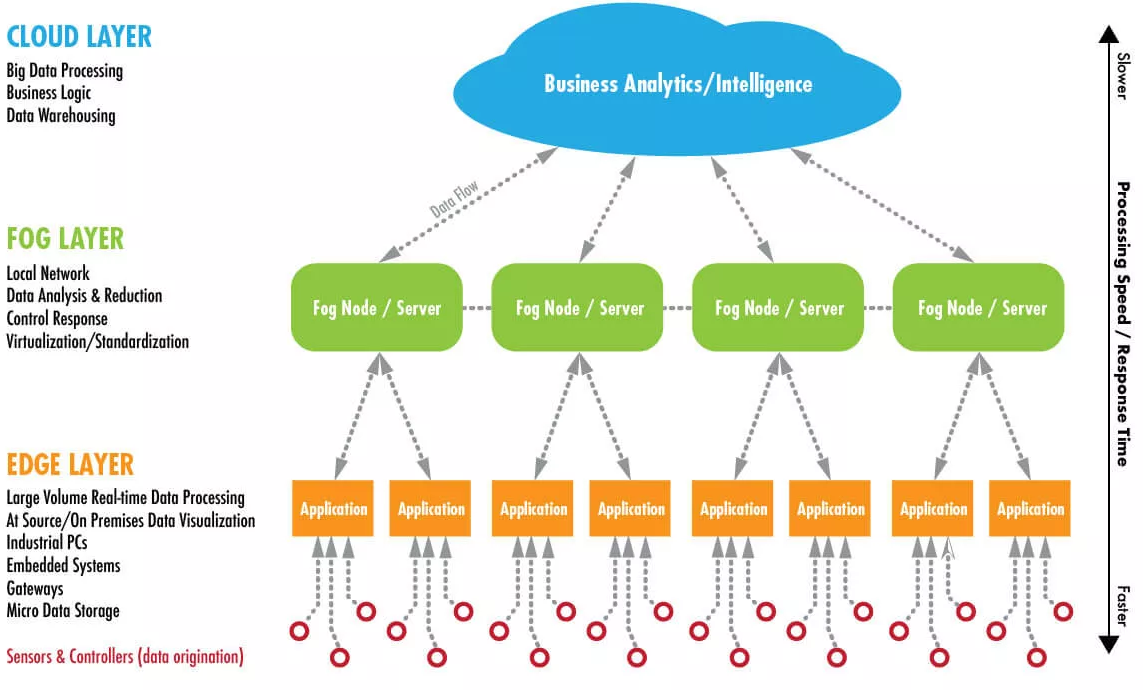
\includegraphics[width=\textwidth]{resources/img/chap2/computing_paradigms}
				\caption{Edge, Fog and Cloud Computing}
				\label{computing_paradigms}
			\end{figure}
		
			Each of these paradigms places computation on a different network layer, from Cloud Computing which lifts off all the need for end devices to compute data, to Edge Computing, where there might be specialized servers physically placed in strategic points so that they are closer to the end devices (lower latency), which may even have the ability to compute data by themselves.
			%https://www.cisco.com/c/en/us/solutions/computing/what-is-edge-computing.html
			On the other hand, Fog Computing is less aggressive than Edge Computing, and does not require the same amount of services placed near the clients, but they can be sorted among the backbone of the network.
			
			These communications do not take place only via Wi-Fi or Ethernet: given that ``\textit{things}'' can be everywhere, the need for a network that can adapt to a fast paced environment is becoming a must.
			Here is where the $5^{th}$ generation of cellular connectivity comes into play.
			
			%https://www.gsma.com/iot/resources/iot-5g-ltem-nbiot-opportunities-benefits/
			As described in a 2019 whitepaper by the GSM Association on IoT and the use of 5G, a ``\textit{combination of 5G and wireless edge technologies will support demanding  use cases, such as autonomous driving, time-critical industrial IoT manufacturing processes and  augmented and virtual reality (AR/VR)}'' \cite{IoT_5g_era}.
			Compared to what is possible with other transmission technologies, 5G supports a massive number in connections, with very little latency.
				
			All of this is not only interesting from a research point of view, but also from a market point of view, where new devices, for consumer and industrial purposes, are created to suit every possible need, that is why IoT can be considered as the ``\textit{next chapter of digital communication}''.
			
			The most notable example from a consumer's point of view, is the smartwatch, which started with the infamous Pebble watch\footnote{ \url{www.kickstarter.com/profile/getpebble/created}}, and is now considered almost a ``\textit{must-have}'' extension of the smartphone.
			Not only it smartwatches can be used for recreational purposes, but some models are crossing the line to becoming medical devices, given the improving accuracy with which they record data.
			Data that, in conjunction with AI, can be used to predict heart attacks \cite{7946780} or other diseases, like Hyperkalemia \cite{HYPERKALEMIA}.
			At the time of writing, IoT devices and frameworks can be used for contact tracing in order to prevent the spread of Covid-19 \cite{9181512}.
			
			Consumers want remote control of simple household devices such as coffee pots so that they may wake up to freshly	brewed coffee, or schedule it to be prepared at a given time.
			% \footnote{ \textit{Hyper Text Coffee Pot Control Protocol}: \url{www.datatracker.ietf.org/doc/html/rfc2324}}.
			
			On the other hand, from an industrial point of view, demands are more focused on fast connectivity among devices, ``\textit{Machine to Machine}'' (M2M), to constantly improve production of goods and services in Industry 4.0 and with the use of Industrial IoT (IIoT).
			% https://www.siemens-advanta.com/blog/what-are-expected-iot-trends-2021
			% IoT is an enabler for the sciences that need large amount of data for creating algorithms and offering better services and more well tailored products.
			The more data available, the more there are opportunities for science, services, business etc. to understand and improve and offer better services and more well tailored products.
			% https://www.mdpi.com/1999-5903/12/3/46
			The growing popularity of IoT use cases in domains that rely on connectivity spanning large areas and the ability to handle a massive number of connections is driving the demand for Low-Power Wide-Area-Network (LPWAN) access technologies, that is why the goal of fifth-generation (5G) wireless networks and beyond is to realize connecting ``\textit{anything, anyone, anytime, anywhere}'' \cite{7414384}.
			LPWANs are better explained in Section \ref{sec:radio_tech}.
			
			Given the importance of this economic sector, many companies, have analyzed the trends and have been producing forecasts about the growth of IoT.
			One analysis, made by The Economist's Intelligence Unit, and sponsored by Arm\footnote{ \url{www.arm.com}}, states that ``\textit{more than two-thirds of respondents agree that understanding the value of data helps them articulate the business case for IoT investments}'' \cite{economist-iot-business-index-2020-arm}.
			In the same analysis, IoT has emerged as an enabler for AI, since many companies ``\textit{view IoT and AI as two components of an advanced analytics capability}'', as previously mentioned.
	
			Underlying hardware challenges such as battery development and energy retention and consumption are among the main research areas that are being investigated, since they represent challenges to the realization of efficient IoT systems.
				
	\section{Air quality}
	
		The ubiquity of mobile technology has opened the door to a new era of mobile sensing. 
		Through this new paradigm that is IoT, physical phenomena can be observed in a distributed way, crowd-sourcing data measurement tasks to smartphones and/or other popular smart wearables.
		Mobile sensing and wireless communications can hence be employed to gather data and generate new information and services, benefitting society.
		Two general strategies can be used to deploy an environmental monitoring system: creating a network of \textit{fixed sensors}	or resorting to \textit{mobile sensors}.
			
		The presence of tiny particulate matter in air is a crucial factor in health, especially when considering urban scenarios.
		In this context, smart mobility coupled with low-cost sensors can create a distributed and sustainable platform for social sensing able to provide pervasive data to citizens and public administrations. 
		Sustainable and eco-aware decisions can then be supported by empirical evidence, resulting in an improved life and better city administration.
		
		Some of the most harmful airborne agents are fine particles (PM2.5), sulphur dioxide (SO2), nitrogen dioxide (NO2), PM10, carbon monoxide (CO), benzene and ozone.
		The maximum amount for these particulates is regulated by various local and international authorities, for example the EU has set standards\footnote{ \url{www.ec.europa.eu/environment/air/quality/standards.htm}} that are reinforced by constant monitoring.
				
		One of the most important instruments in air quality measurement is the \textit{Keeling Curve}: a meticulous record of the amount of carbon dioxide in the atmosphere.
	
		\noindent
		\begin{minipage}{0.49\textwidth}%
			\begin{figure}[H]
				\centering
				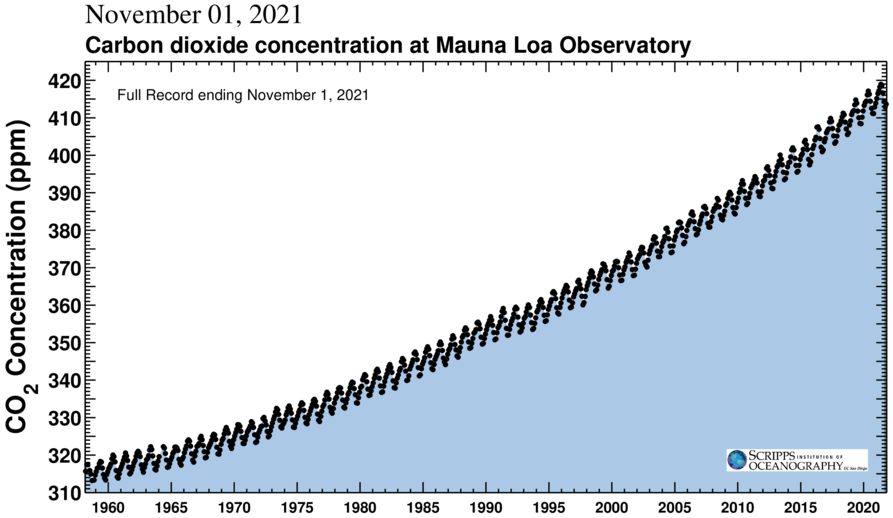
\includegraphics[width=\textwidth]{resources/img/chap2/keeling}
				\caption{Full record Keeling curve until Nov. 1 2021}
				\label{keeling_full}
			\end{figure}
		\end{minipage}%
		\hfill%
		\begin{minipage}{0.49\textwidth}\raggedright
			\begin{figure}[H]
				\centering				
				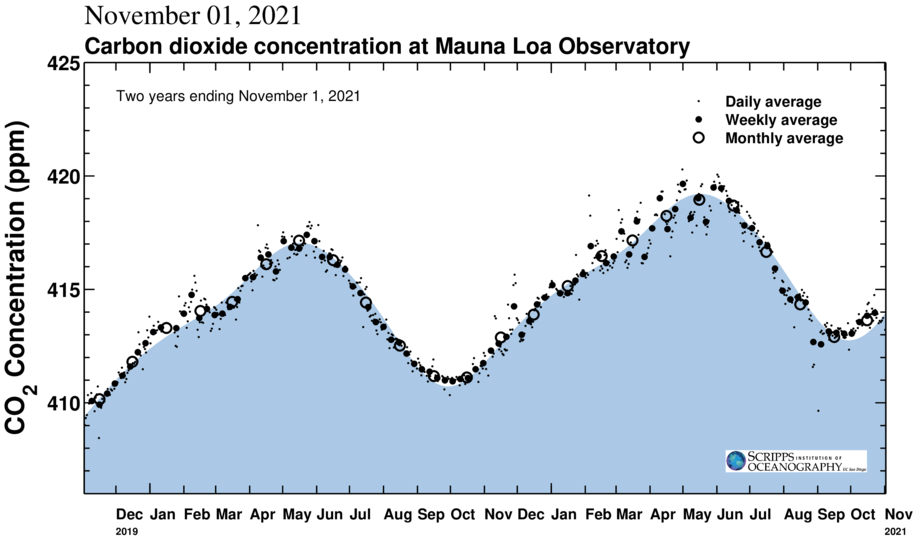
\includegraphics[width=\textwidth]{resources/img/chap2/mlo_two_years}
				\caption{Two years Keeling curve until Nov. 2021}
				\label{keeling_two}
			\end{figure}
		\end{minipage}
		\newline
		
		The Keeling Curve tracks changes in the concentration of CO2 in the Earth's atmosphere using data from a research station on Mauna Loa, Hawaii.
		Figure~\ref{keeling_full} shows the result of daily readings that have continued almost uninterrupted for more than 60 years, while Figure~\ref{keeling_two} shows the data between October 2019 and November 2021.
		The importance of this instrument lies in the fact that, over those six decades, the zig-zag has trended steadily upward. 
		Real time readings can be found on the UC San Diego, Institution of Oceanography's dedicated website\footnote{ \url{keelingcurve.ucsd.edu}}.
		
		Many projects have been made, both for research and commercial purposes, to detect pollutants in the air and raise awareness of the conditions people are living in.
		Below are two research solutions that have been made for air quality sensing with low-cost sensors.
			
		\subsection{ArduECO}\label{subsec:ardueco}
			% https://www.hackster.io/news/nodemcu-based-ardueco-aims-to-track-global-air-quality-metrics-using-bike-sharing-fleets-75d50e169fc8
			% https://www.math.unipd.it/~cpalazzi/ArduECO/ArduECO%20IEEE%20Presentation%20FINAL.pdf
			% https://arxiv.org/pdf/2007.08305.pdf
			
			ArduECO is a wireless device based on an Arduino-like board, esp8266, capable of gathering data about air quality (and more with simple extensions) and sending them to the cloud, to be processed and displayed.

			This solution has been proposed in the paper ``\textit{Air Quality Control through Bike Sharing Fleets}''\cite{ardueco_paper}, presented at the 2020 IEEE Symposium on Computers and Communications.
			
			\begin{figure}[h]
				\centering
				\includegraphics[width=.9\textwidth]{resources/img/chap2/ardueco_circuit}
				\caption{Circuit of the ArduECO prototype}
				\label{img:ardueco_circuit}
			\end{figure}
			
			One of the main design goals of this device is to be easily fit on shared means of transportation, such as bikes and electric scooters, which been advantaged by the COVID-19 pandemic \cite{HU2021102997}, contrast other shared transportation approaches, such as car sharing, that have severely suffered from the pandemic.
			
			ArduECO is built around four core components: the NodeMCU ESP8266-based development board, a microSD card reader for local data caching, a GPS-based global navigation satellite system receiver for location data and an MQ-7 carbon monoxide (CO) sensor, which can easily be replaced with other sensors using the same pinout.
			Figure~\ref{img:ardueco_circuit} shows the full circuit of the prototype, while Figure~\ref{img:ardueco_picture} is a picture of the built device.
			
			As well as capturing the air quality data locally, data is cached and later sent in the cloud to an MQTT server running on Amazon Web Services IoT Core.
			
			\noindent
			\begin{minipage}{0.38\textwidth}
				\begin{figure}[H]
					\centering
					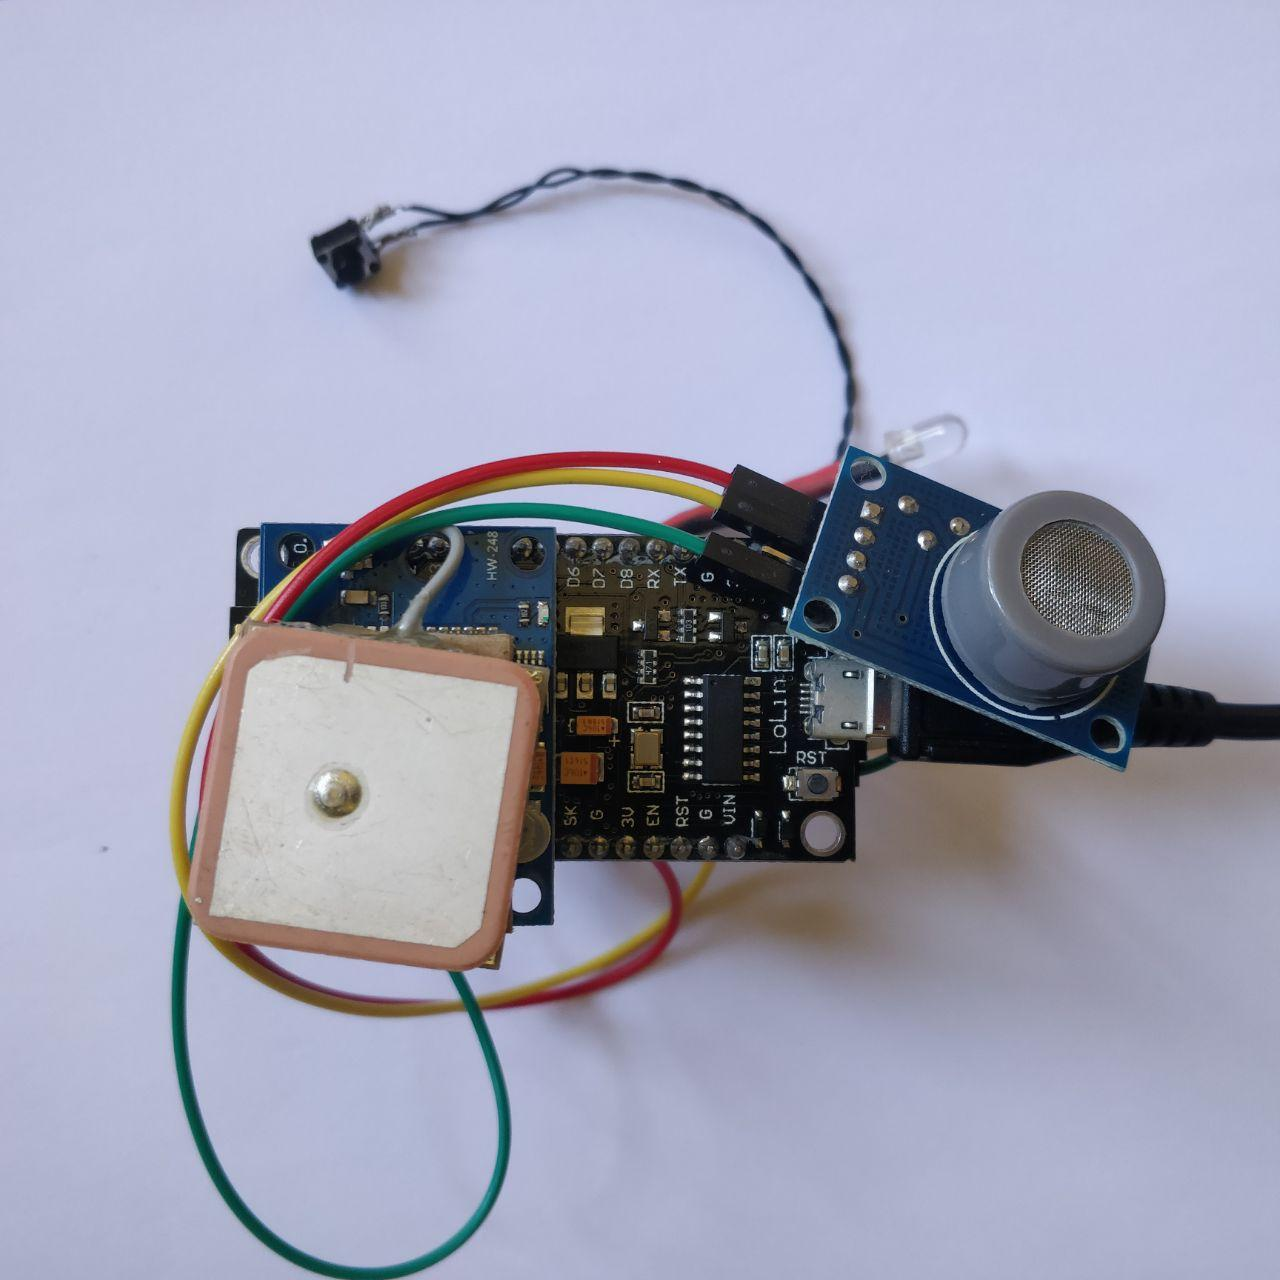
\includegraphics[width=\textwidth]{resources/img/chap2/ardueco_picture}
					\caption{Built ArduECO prototype}
					\label{img:ardueco_picture}
				\end{figure}
			\end{minipage}%
			\hfill%
			\begin{minipage}{0.6\textwidth}\raggedright
				Server costs aside, the sensor platform can be built in a bill of materials of around $15$€, or less if the materials are bought in bulk.
				
				As described in the paper, this project is more of a proof of concept that shows the possibility of creating a small and cheap device which can be placed on shared means of transportation.
				Therefore there are various aspects that can be improved, such as adding multiple sensors to detect different pollutants and tweak the software so that the board can sleep and save battery.
			\end{minipage}

		\subsection{MegaSense}\label{subsec:megasense}
	
			% https://www.researchgate.net/profile/Samu-Varjonen
	
			% https://www.megasense.org/
			% https://uia-initiative.eu/en/uia-cities/helsinki	
			% https://ieeexplore.ieee.org/document/9248143
		
			MegaSense is a project that has been developed by the Departments of Computer Science at the University of Helsinki\footnote{ \url{www.helsinki.fi/en/computer-science}} and brings forward accurate portable low-cost sensing devices and an online data platform integrating multiple sources of urban data and leveraging AI network calibration producing hyper-local air quality information in real time.
				
			Compared to the previously described ArduECO, MegaSense, represented in Figure~\ref{img:megasense_picture}, is a more complete project which has been tested by citizens and companies in City of Helsinki and EU projects.
			It is also encased in a $3$D printed case and has an rechargeable battery, allowing it to be immediately given to the users.

			The back-end system receives data from sensing platforms, the individual MegaSense devices, measuring local pollution exposure and other variables affecting it.
			These data are processed into air quality information such as maps and advice on how to reduce personal exposure, take healthier routes, and direct participants to improve measurements in areas that have limited sensor coverage.
			
			\noindent
			\begin{minipage}{0.35\textwidth}
				\begin{figure}[H]
					\centering
					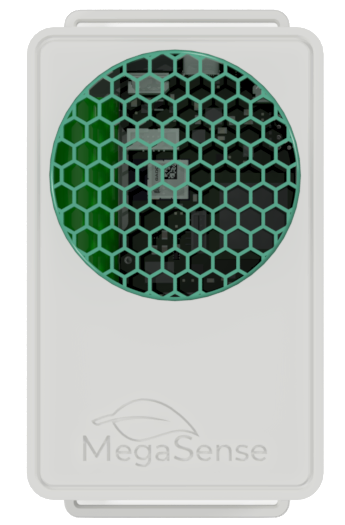
\includegraphics[width=.8\textwidth]{resources/img/chap2/megasense}
					\caption{MegaSense prototype}
					\label{img:megasense_picture}
				\end{figure}
				\vspace{3mm}
			\end{minipage}%
			\hfill%
			\begin{minipage}{0.65\textwidth}\raggedright
				As explained in the main paper \cite{megasense} regarding this device, ``\textit{the core of MegaSense consists of two layers: the Edge and Cloud}''.
				The Edge layer receives data from available node and delivers pollution maps to the mobile app, which provides users with personal air pollution exposure	information as well as local exposure maps.
				This layer is responsible for data pre-processing, filtering and data cleaning.
				The Cloud layer, which runs on AWS, is responsible for storing cleaned data	and aggregating the crowd-sourced data while preserving the privacy of participants.
			\end{minipage}

			Registered citizens that have been given the device, download the HOPE Exposure App from Google play store and tether their Android smart phone to the sensor.
			The phone gathers data from the sensor, alongside the GPS coordinates, and it sends them in the cloud.
			
			This project develops the clean air journey	planner application that creates optimal walking and cycling routes based on air quality of Helsinki.